\documentclass[../main.tex]{subfiles}

\begin{document}

\section{Question 1} \label{sec:q1}

Calculation of the inverse of a 2 by 2 matrix is shown below.

$$
A =
\begin{bmatrix}
    a & b \\
    c & d
\end{bmatrix}
, \hspace{20pt} A^{-1} = \frac{1}{|A|}
\begin{bmatrix}
    d & -b \\
    -d & a
\end{bmatrix}
= \frac{1}{ad - bc}
\begin{bmatrix}
    d & -b \\
    -c & a
\end{bmatrix}
=
\begin{bmatrix}
    a_\text{out} & b_\text{out} \\
    c_\text{out} & d_\text{out}
\end{bmatrix}
$$

You are to design an RTL circuit for this calculation. When \texttt{start} is asserted, \texttt{aIn}, \texttt{bIn}, \texttt{cIn}, \texttt{dIn} 16-bit busses will contain the four elements of the matrix in upper left to lower right order. When the inverse calculation is completed, the IMC (Inverse Matrix Calculator) generates a 1 on \texttt{ready} and keeps this value until a new round of calculation begins. When calculation is completed, the output data becomes available on \texttt{aOut}, \texttt{bOut}, \texttt{cOut}, \texttt{dOut} output busses. Input and output data formats are 16-bit fixed point with eight integer bits. The inputs have only integer parts, and the outputs are 16-bit data with integer and fractional parts. The input integer part should be less than or equal to 15.

You can use the following components:

\begin{itemize}
    \item 2 16-bit unisgned multipliers with 16-bit inputs and a 16-bit outputs. Each has a control signal, \texttt{select\_output}, which determines which portion of the 32-bit multiplication result is select: when $\texttt{select\_output} = 1$, the most significant 16 bits are chosen, otherwise, the bits in the range $[23:8]$ are selected. Consider the delay of this multiplier is in the order of 84d.
    \item An approximate reciprocal circuit with an unsigned 16-bit integer input and 9-bit output (1-bit integer and an 8-bit fractional). The circuit is combinational, calculates the reciprocal of its input, and has a delay of 84d.
    \item 16-bit adders, subtractors, and comparators with delay values of the order 16d.
    \item Multiplexers, decoders, and other combinational parts with delay values of the order of 1d.
    \item Registers of any size.
\end{itemize}

Design the IMC circuit such that it can operate with a clock with a period of \textbf{no more than 120d}. This limits the maximum critical path delay the circuit can have. For outputs that are negative produce a negative flag of 1.

\begin{enumerate}
    \item Create behavioural models for the multipliers and adder/subtractor.
    \item Draw the complete datapath of IMC, including the components and necessary internal control signals.
    \item Draw a state diagram showing your controller's behaviour. In each state, show the control signals that are issued.
    \item Show wiring between the datapath and the controller.
    \item Model the IMC circuit in SystemVerilog according the the schematic, datapath, and controller. \textbf{You don't need to model the delays.}
    \item Verify the design with a testbench.
\end{enumerate}

\newpage

\subsection*{Solution}

\begin{figure}[h]
    \centering
    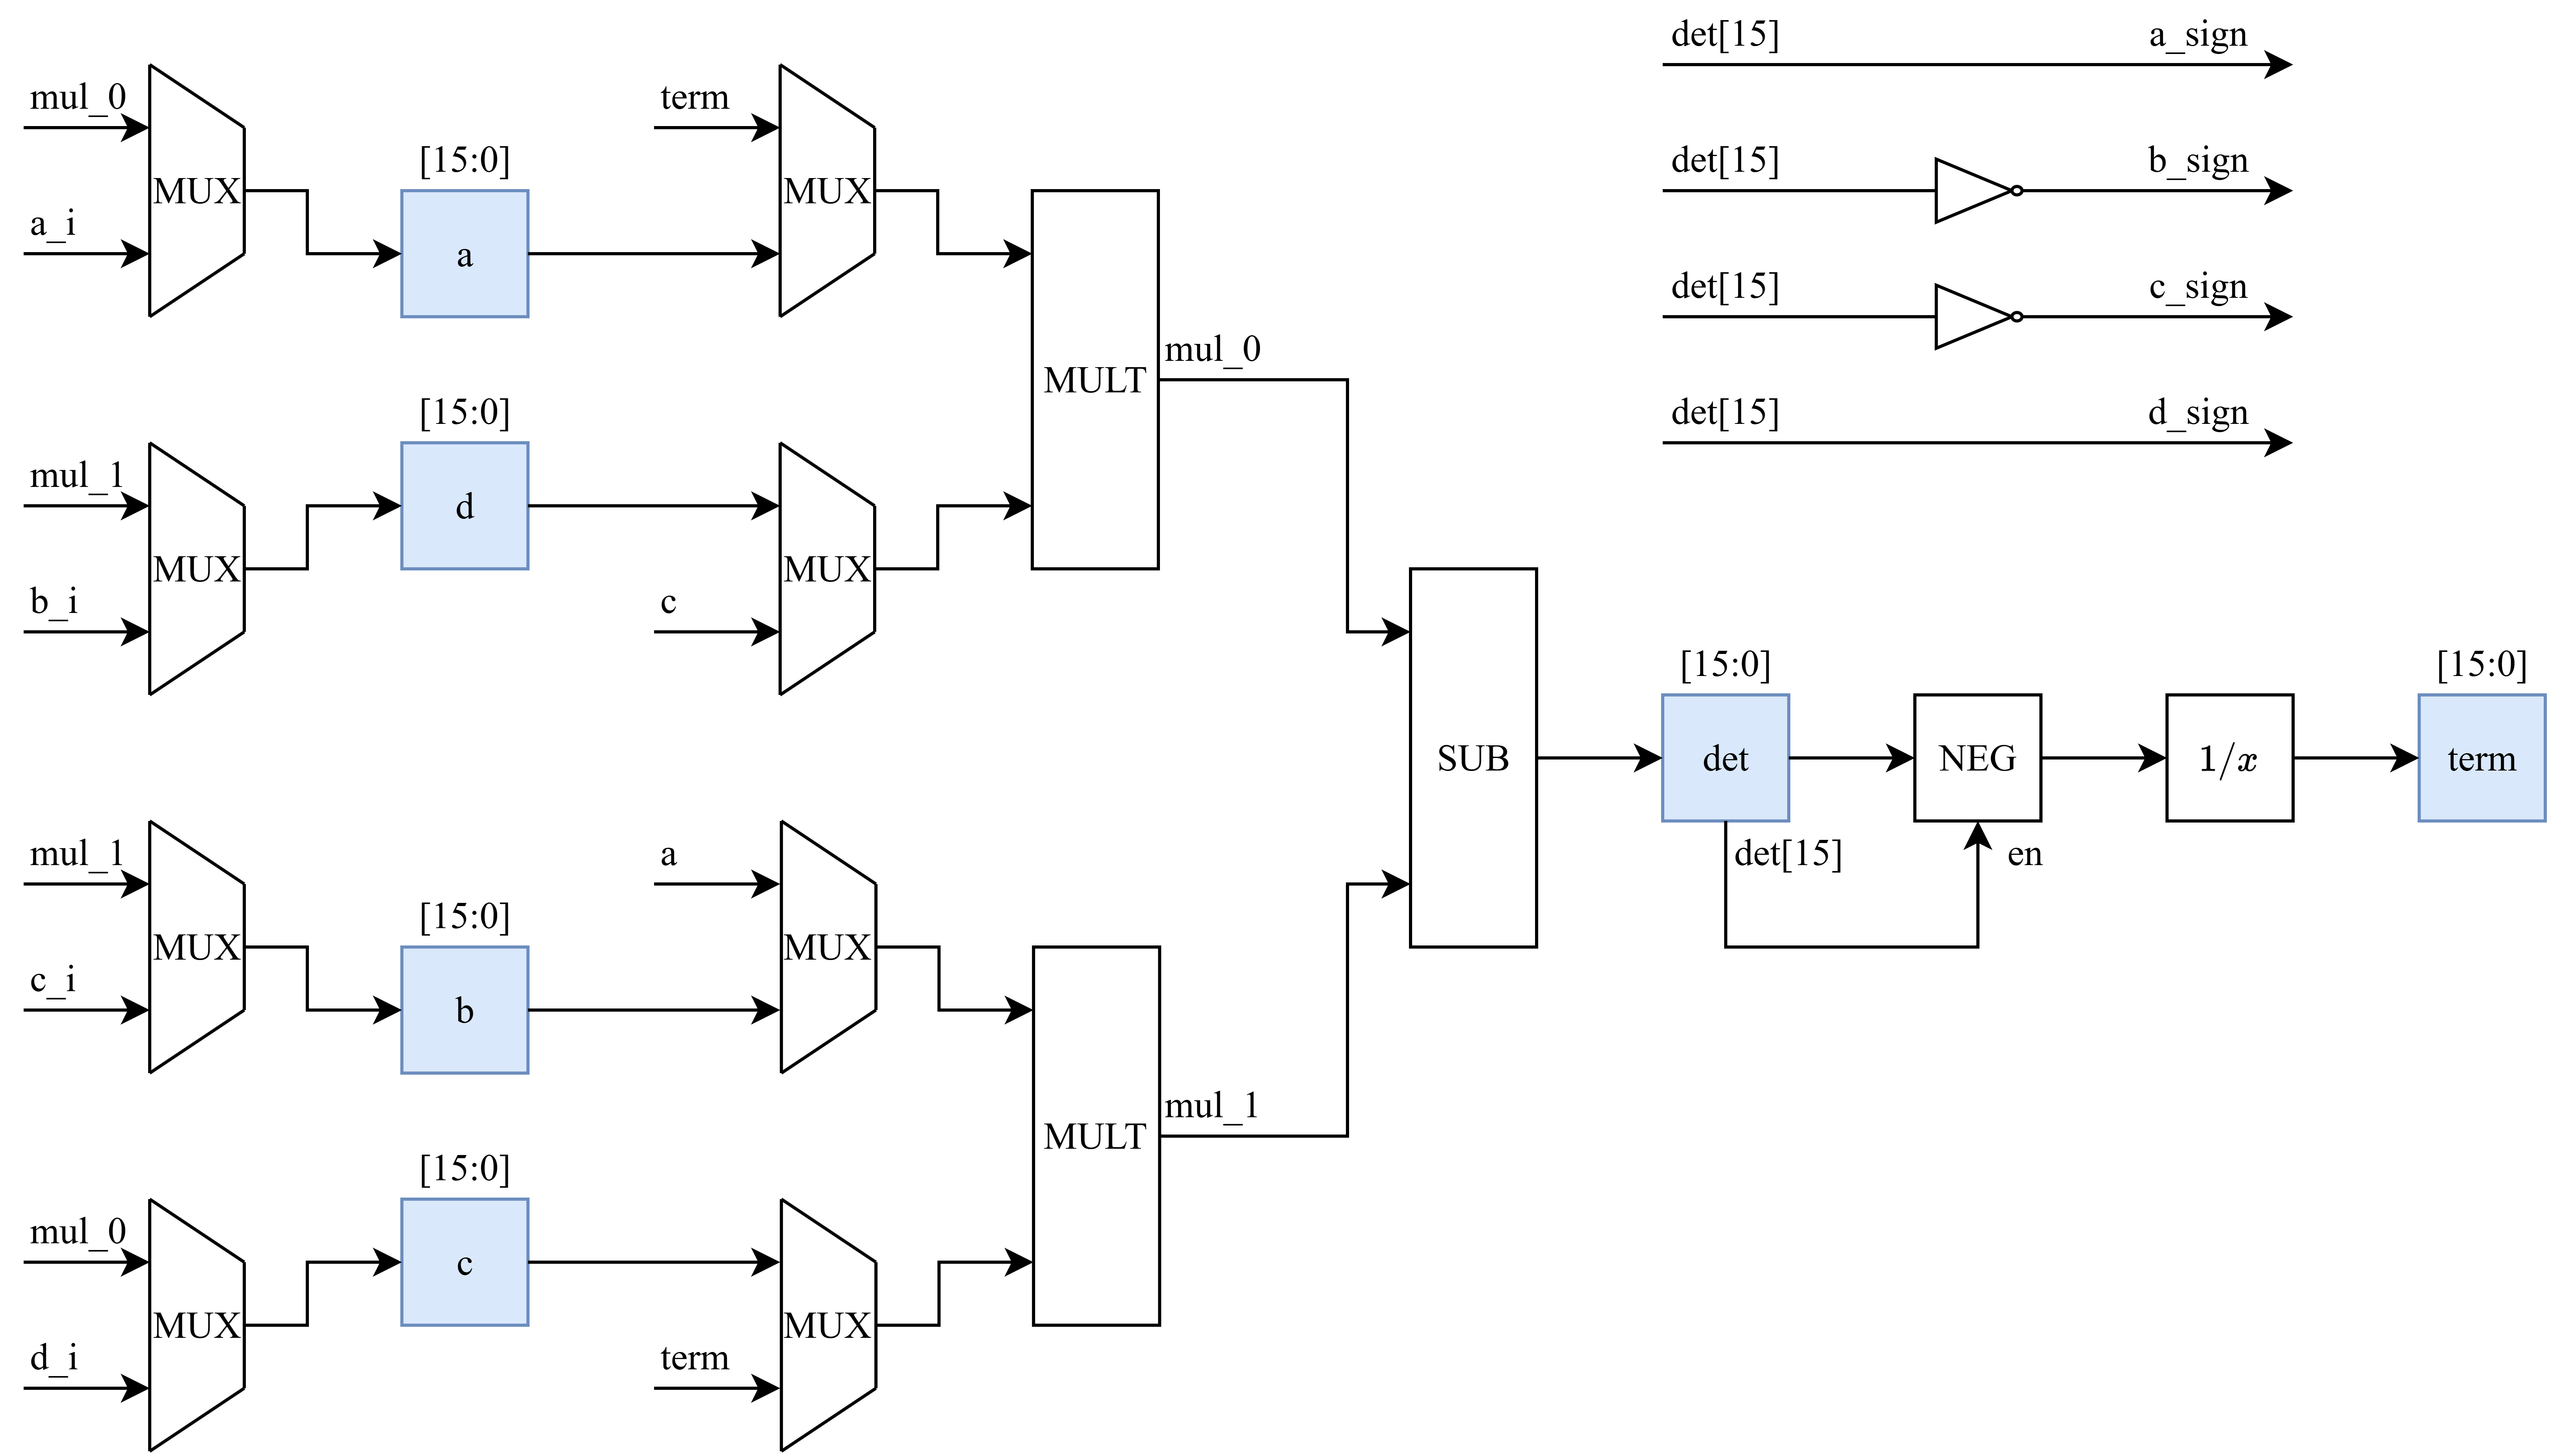
\includegraphics[width=\linewidth]{assets/q1.png}
    \caption{Datapath of IMC module. Registers are shown in blue.}
    \label{fig:q1_dp}
\end{figure}

To construct the \textit{Inverse Matrix Calculator} (IMC), we utilize 8 multiplexers, two multipliers, two adders, and one reciprocal module. To comply with the timing specifical of a maximum critical path delay of 120d, we have 6 registers (shown in blue). The datapath schematic is shown in \cref{fig:q1_dp}. The calculation consists of 5 steps corresponding directly to 5 clock cycles [\cref{tab:pipeline_cycles}].

\begin{table}[h]
    \centering
    \renewcommand{\arraystretch}{1.5}
    \setlength{\tabcolsep}{8pt}
    \begin{tabularx}{\textwidth}{@{}cX@{}}
        \toprule
        \textbf{Cycle} & \textbf{Operation} \\
        \midrule
        0 & Input values are clocked into the input/output registers \texttt{a}, \texttt{b}, \texttt{c}, and \texttt{d}. \\
        1 & The determinant, $ad - bc$, is calculated and stored in \texttt{det}. \\
        2 & If the determinant is negative, it is negated (subtractor with one operand set to 0) and the reciprocal is computed and stored in \texttt{term}. \\
        3 & Half of the inverse matrix, \texttt{aOut} and \texttt{dOut}, is computed and stored in the \texttt{a} and \texttt{d} registers. \\
        4 & The second half of the inverse matrix, \texttt{bOut} and \texttt{cOut}, is computed and stored in the \texttt{b} and \texttt{c} registers. \\
        \bottomrule
    \end{tabularx}

    \caption{Pipeline operation by clock cycle.}
    \label{tab:pipeline_cycles}
\end{table}

The sign of each entry in the inverse matrix result is computed directly from the sign of the determinant. The control signals needed for the datapath are summarized in \cref{tab:q1_control}. They consist entirely of 1-bit signals to control the registers and muxes. The longest path delay consists of the route from the input registers to the \texttt{det} register with a total delay of $1d + 84d + 16d = 101d$. The controller has a total of 7 states. Their transitions are shown in \cref{fig:q1_controller}.

\newpage

\begin{table}[h]
    \centering
    \renewcommand{\arraystretch}{1.2}
    \setlength{\tabcolsep}{8pt}

    \begin{tabularx}{\textwidth}{@{}lX@{}}
        \toprule
        \textbf{Signal} & \textbf{Description} \\
        \midrule
        \texttt{en\_a}          & Enable synchronized writing into the \texttt{a} register. \\
        \texttt{en\_b}          & Enable synchronized writing into the \texttt{b} register. \\
        \texttt{en\_c}          & Enable synchronized writing into the \texttt{c} register. \\
        \texttt{en\_d}          & Enable synchronized writing into the \texttt{d} register. \\
        \texttt{en\_det}        & Enable synchronized writing into the \texttt{det} register. \\
        \texttt{en\_term}       & Enable synchronized writing into the \texttt{term} register. \\
        \texttt{sel\_a}         & Input register mux. 1'b0: \texttt{a\_i}, \hspace{20pt} 1'b1: \texttt{mul\_0}. \\
        \texttt{sel\_b}         & Input register mux. 1'b0: \texttt{b\_i}, \hspace{20pt} 1'b1: \texttt{mul\_1}. \\
        \texttt{sel\_c}         & Input register mux. 1'b0: \texttt{c\_i}, \hspace{20pt} 1'b1: \texttt{mul\_0}. \\
        \texttt{sel\_d}         & Input register mux. 1'b0: \texttt{d\_i}, \hspace{20pt} 1'b1: \texttt{mul\_1}. \\
        \texttt{sel\_mul\_a\_0} & Multiplier 0 mux. \hspace{5pt} 1'b0: \texttt{a}, \hspace{35pt} 1'b1: \texttt{term}. \\
        \texttt{sel\_mul\_b\_0} & Multiplier 0 mux. \hspace{5pt} 1'b0: \texttt{b}, \hspace{35pt} 1'b1: \texttt{c}. \\
        \texttt{sel\_mul\_a\_1} & Multiplier 1 mux. \hspace{5pt} 1'b0: \texttt{c}, \hspace{35pt} 1'b1: \texttt{a}. \\
        \texttt{sel\_mul\_b\_1} & Multiplier 1 mux. \hspace{5pt} 1'b0: \texttt{d}, \hspace{35pt} 1'b1: \texttt{term}. \\
        \bottomrule
    \end{tabularx}

    \caption{Control signals for IMC datapath.}
    \label{tab:q1_control}
\end{table}

\vspace{-10pt}
\begin{figure}[h]
    \centering
    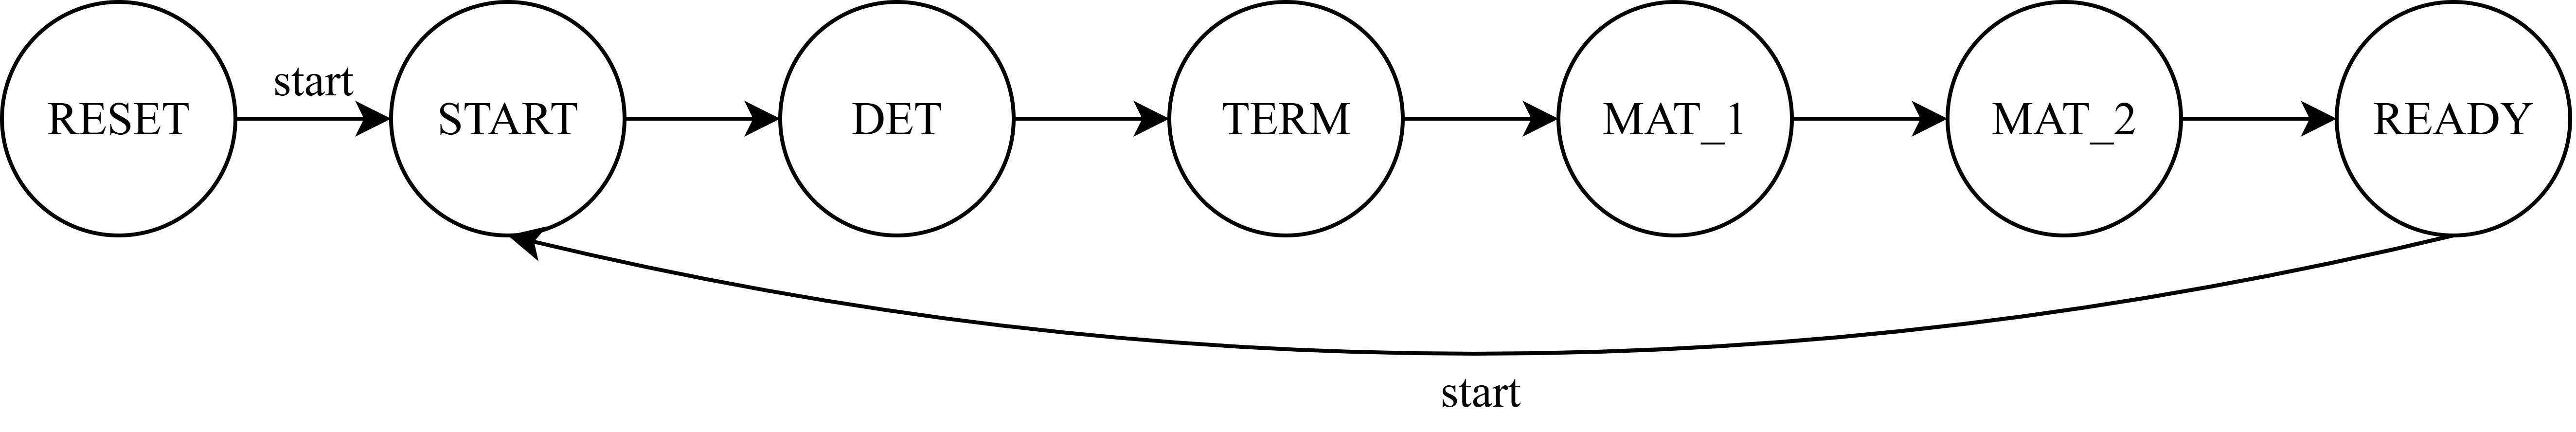
\includegraphics[width=\linewidth]{assets/q1_state.png}
    \caption{State transition diagram for IMC controller.}
    \label{fig:q1_controller}
\end{figure}

% \vspace{-10pt}
The control signals issued in each state are summarized in \cref{tab:q1_state_signals}. Finally for verification we create a testbench that input all combinations of integer values in the range $[0, 15]$ and check the result against a software implementation. It is important to note that for input values that result in a determinant above 15, the given reciprocal module doesn't work anymore and gives invalid values. Therefore such tests are skipped. A snippet of the testbench output is shown below. It passes with 0 errors with a tolerance of $0.041$ against the true software result.

\begin{textcode}{q1 - IMC testbench output}
Matrix: [[15, 9], [6, 3]]
HW inv: [-0.3281, 0.9844; 0.6562, -1.6406]
Ref inv: [-0.3333, 1.0000; 0.6667, -1.6667]

Matrix: [[15, 9], [6, 4]]
HW inv: [0.6562, -1.4766; -0.9844, 2.4609]
Ref inv: [0.6667, -1.5000; -1.0000, 2.5000]

...

[861270] Completed with 0 errors...
\end{textcode}

\newpage

\begin{table}[h]
    \centering
    \renewcommand{\arraystretch}{1.5}
    \setlength{\tabcolsep}{6pt}

    \begin{tabularx}{\textwidth}{@{}l X@{}}
        \toprule
        \textbf{State} & \textbf{Signals Active (1'b1)} \\
        \midrule
        \texttt{STATE\_START} & 
            \texttt{en\_a\_o} \newline
            \texttt{en\_b\_o} \newline
            \texttt{en\_c\_o} \newline
            \texttt{en\_d\_o} \\
        \hline
        \texttt{STATE\_DET} & 
            \texttt{en\_det\_o} \\
        \hline
        \texttt{STATE\_TERM} & 
            \texttt{en\_term\_o} \\
        \hline
        \texttt{STATE\_MAT\_1} & 
            \texttt{en\_a\_o} \newline
            \texttt{en\_d\_o} \newline
            \texttt{sel\_a\_o} (mul\_0) \newline
            \texttt{sel\_d\_o} (mul\_1) \newline
            \texttt{sel\_mul\_a\_0\_o} (term) \newline
            \texttt{sel\_mul\_a\_1\_o} (a) \newline
            \texttt{sel\_mul\_b\_1\_o} (term) \\
        \hline
        \texttt{STATE\_MAT\_2} & 
            \texttt{en\_b\_o} \newline
            \texttt{en\_c\_o} \newline
            \texttt{sel\_b\_o} (mul\_1) \newline
            \texttt{sel\_c\_o} (mul\_0) \newline
            \texttt{sel\_mul\_a\_0\_o} (term) \newline
            \texttt{sel\_mul\_b\_0\_o} (c) \newline
            \texttt{sel\_mul\_b\_1\_o} (term) \\
        \hline
        \texttt{STATE\_READY} & 
            \texttt{ready\_o} \\
        \bottomrule
    \end{tabularx}

    \caption{Signals issued in each state.}
    \label{tab:q1_state_signals}
\end{table}

\newpage

\section{Question 2}

In this problem, you are to design an input wrapper and an output wrapper that connect the IMC circuit of the previous problem to a 16-bit arbitrated bus.

The input wrapper waits for four 16-bit data that will be handshaked to it using a two-line \texttt{dataReady}, \texttt{dataAccept} fully responsive handshaking scheme. When such is received, it checks if the IMC circuit is ready to receive its four 16-bit inputs by monitoring the IMC's \texttt{ready} output. If so, it issues a \texttt{start} signal and allows the IMC to start its operation.

The output wrapper works independently of the input wrapper. the output wrapper receives the four outputs of the IMC circuit when the IMC issues the \texttt{ready} signal. The output wrapper has an \texttt{outAvail} output that informs an external device of the availability of four 16-bit elements of the transposed matrix. When this signal is asserted, the external device may issue a start signal, \texttt{startTransmit}, to tell the output wrapper to start sending the results. The output wrapper uses \texttt{request} to get permission to use the bus, that will be responded by \texttt{grant} when the output wrapper is allowed to drive the bus. The output wrapper uses fully responsive two-line handshaking using an \texttt{outReady} output and an \texttt{outAccepted} input. The four 16-bit data outputs will be sent over the bus ina  burst fashion.

\begin{enumerate}
    \item Draw block diagrams of the input wrapper, output wrapper, and the interfacing bus, and how they wrap around the IMC circuit.
    \item Draw the datapath of the interfacing circuits, identifying control signals that are issued by the controller.
    \item Draw the state machines for the implementation of the inerface circuits controller.
    \item Model your input wrapper and output wrapper in SystemVerilog.
    \item verify your design with a testbench.
\end{enumerate}

\subsection*{Solution}



\end{document}
